% Task 3 – Thiết kế kiến trúc
% Nguồn: docs/architecture/architecture.md, deployment-view.md, adr/*.md, diagrams/*.puml
\section{Task 3 -- Thiết kế kiến trúc}\label{sec:architecture}

%%%%%%%%%%%%%%%%%%%%%%%%%%%%%%%%%%%%%%%%%%%%%%%%%%%%%%%%%%%%%%%%%%%%%%
\subsection{Task 3.1 -- Phương pháp và quyết định kiến trúc}

\subsubsection{Phương pháp}
Kiến trúc được mô tả theo \textbf{mô hình C4} ở ba mức (System Context, Container, Component). Bên trong mỗi module
backend áp dụng \textbf{kiến trúc phân lớp}. Mọi sơ đồ nằm trong \code{docs/architecture/diagrams/} (\code{.puml} và
\code{.svg}); mô tả đầy đủ ở \code{docs/architecture/architecture.md}.

\begin{figure}[H]
\centering
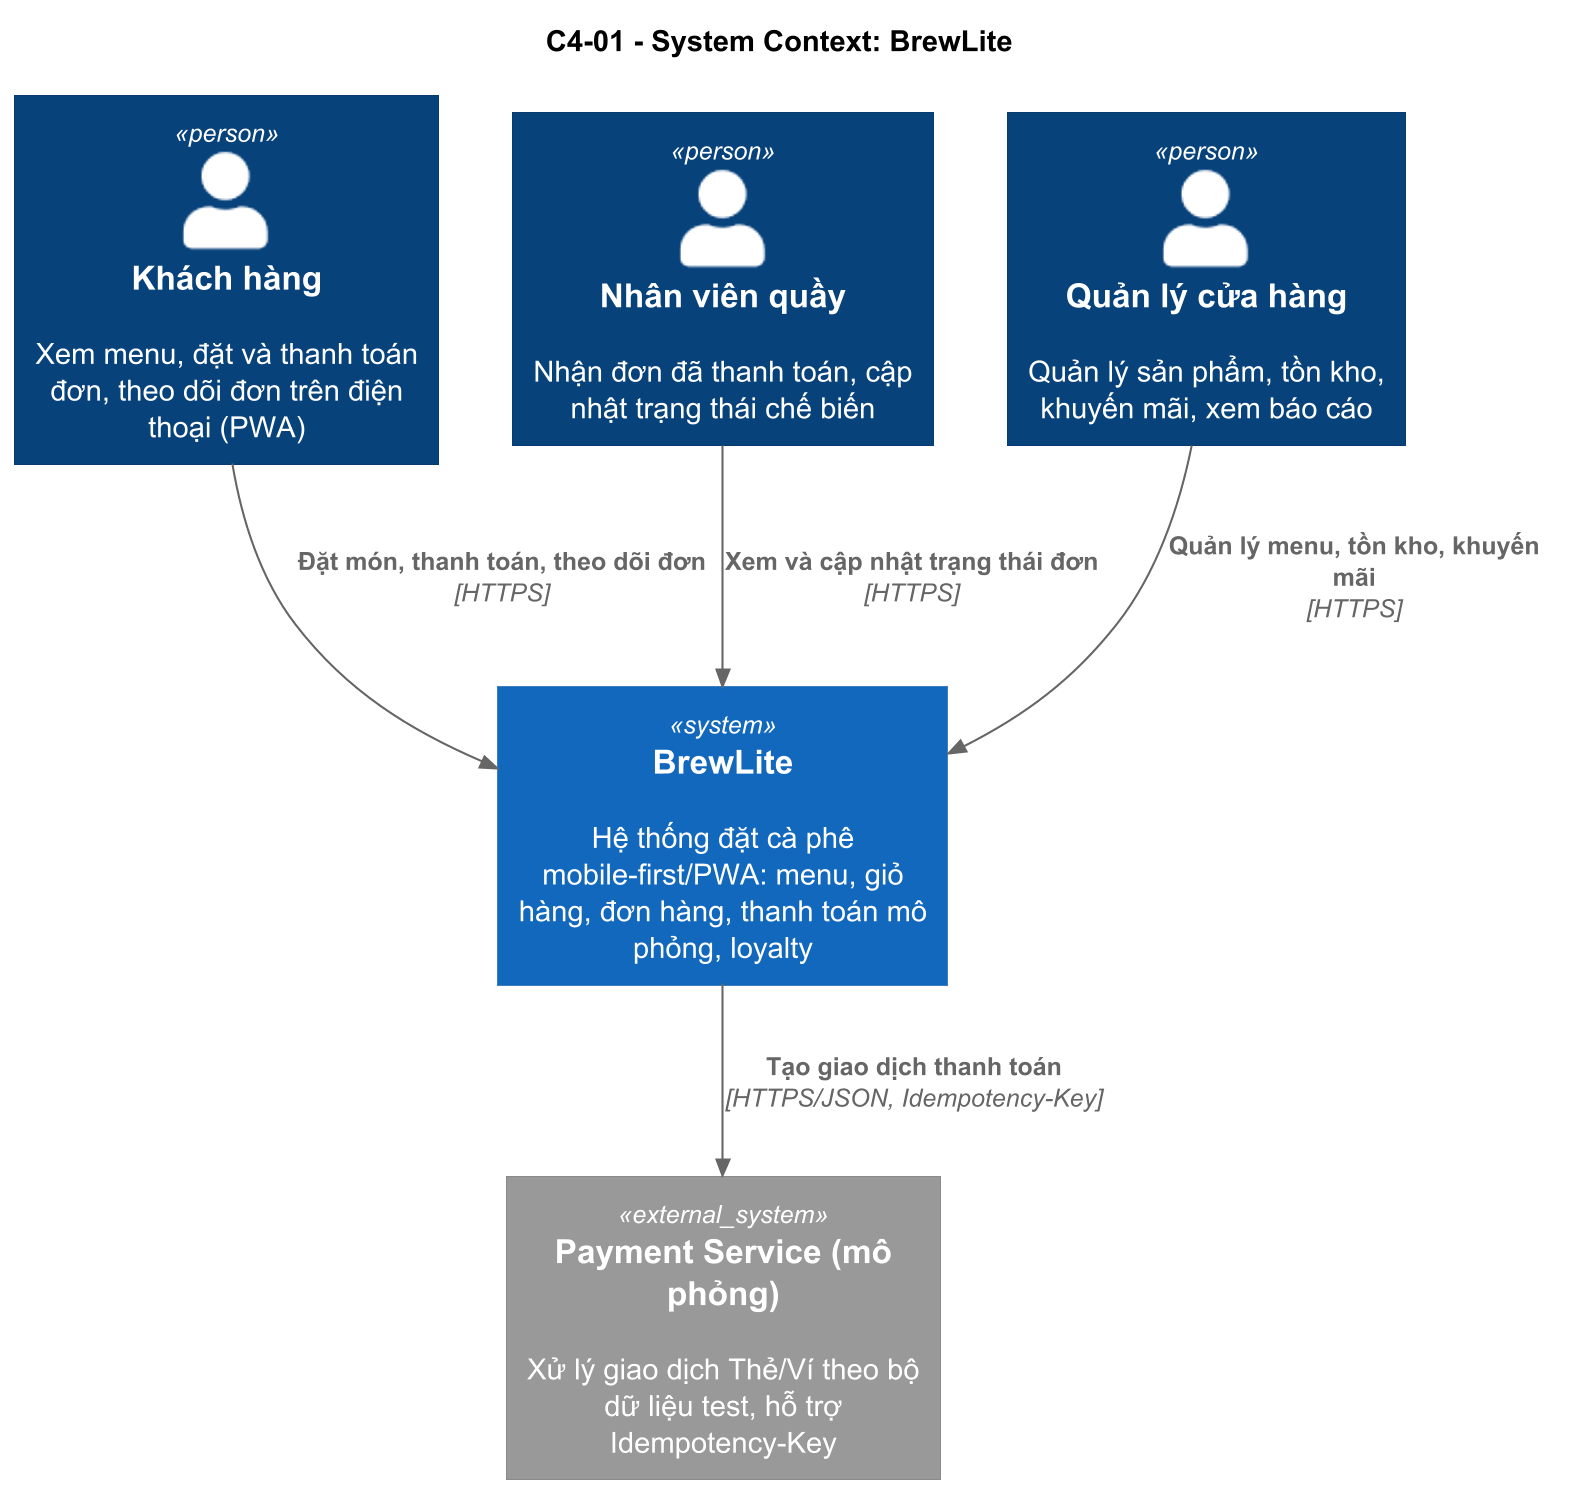
\includegraphics[width=0.72\textwidth]{figures/c4-context.png}
\caption{C4-01 -- System Context của BrewLite}\label{fig:c4-context}
\end{figure}

\begin{figure}[H]
\centering
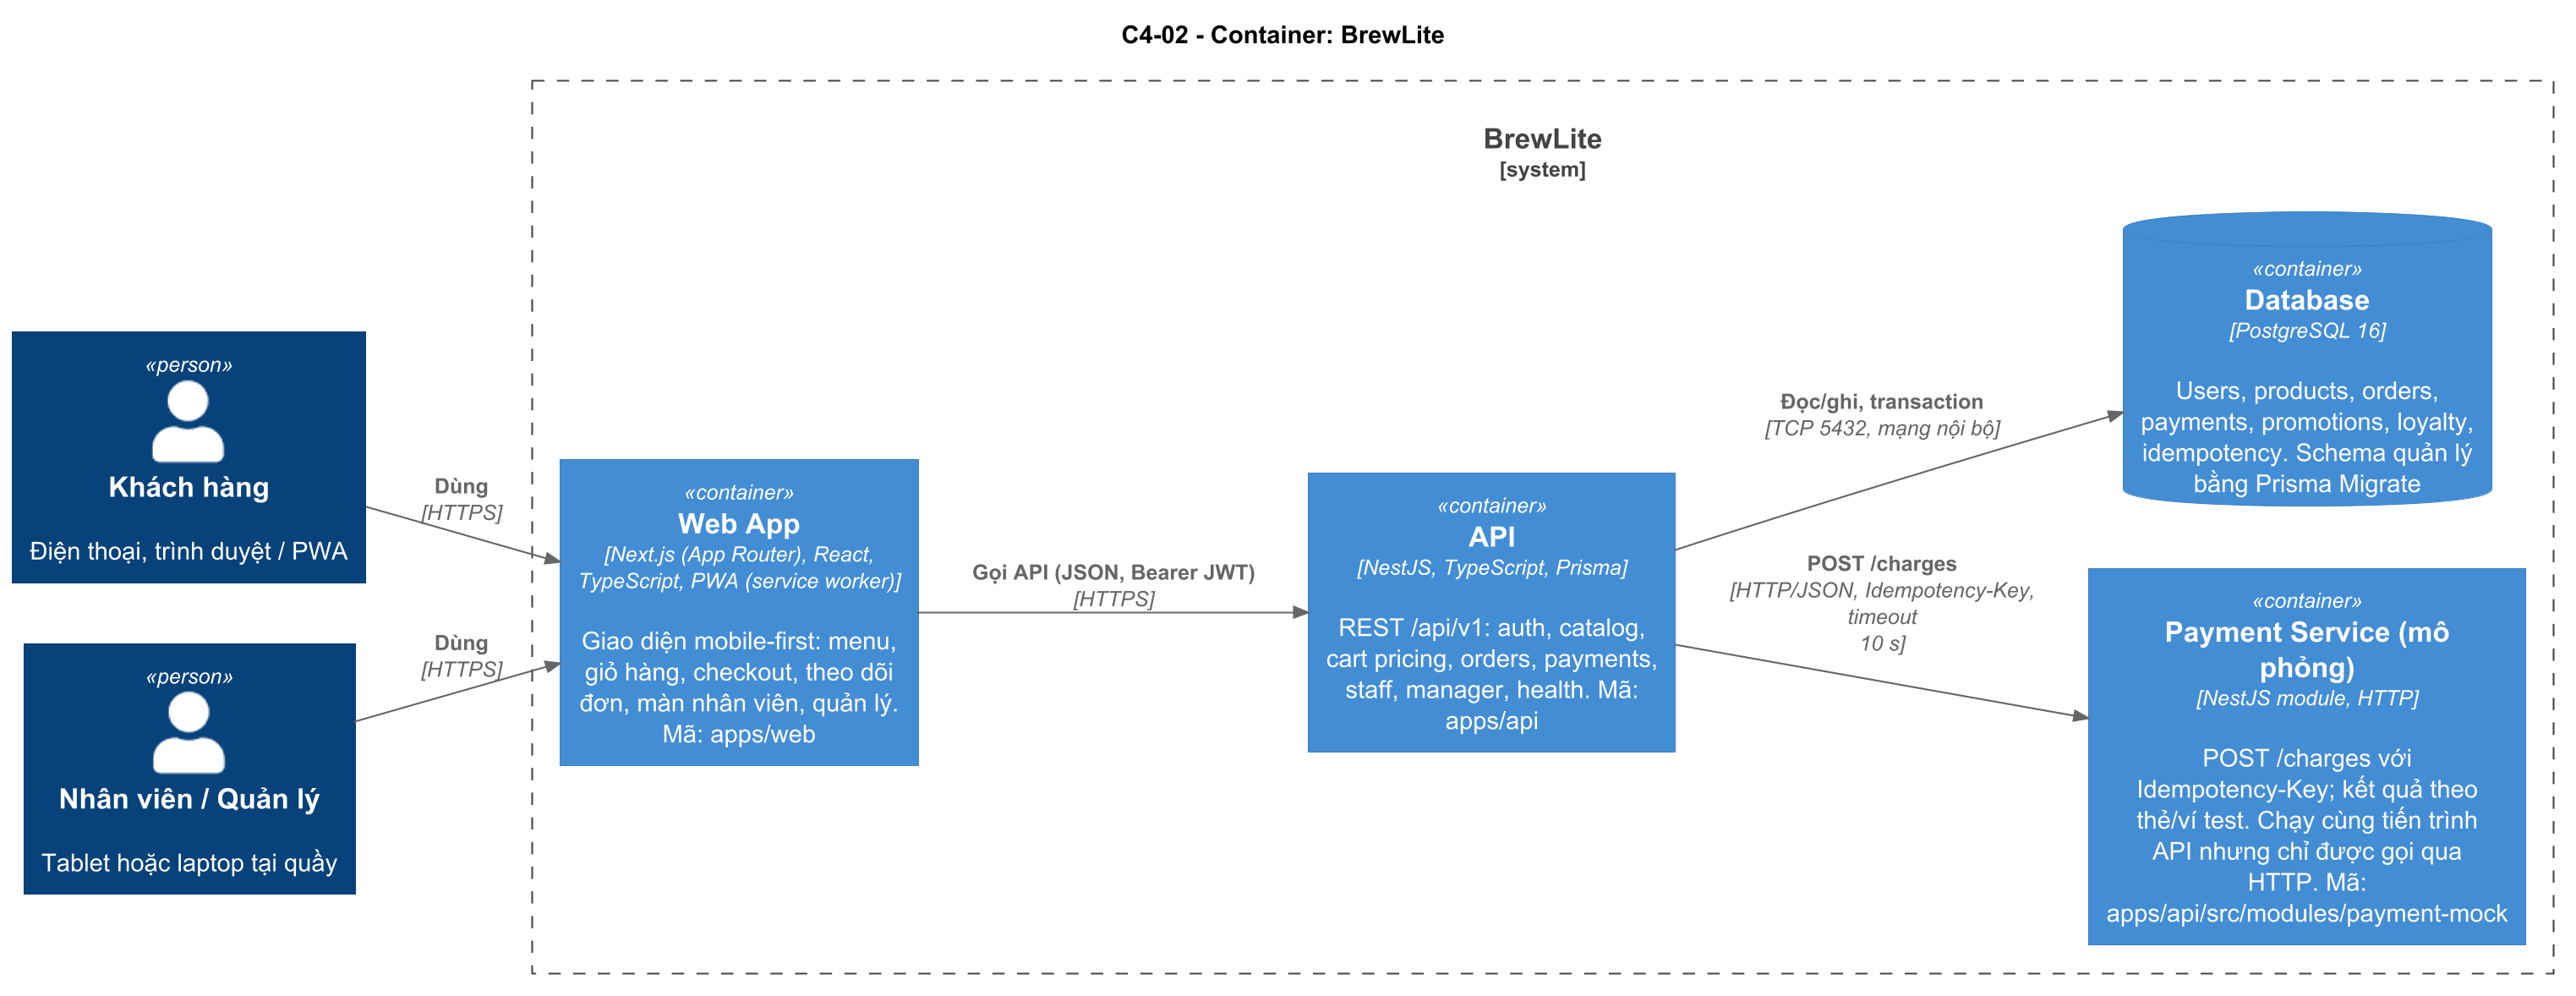
\includegraphics[width=\textwidth]{figures/c4-container.png}
\caption{C4-02 -- Container của BrewLite}\label{fig:c4-container}
\end{figure}

\begin{figure}[H]
\centering
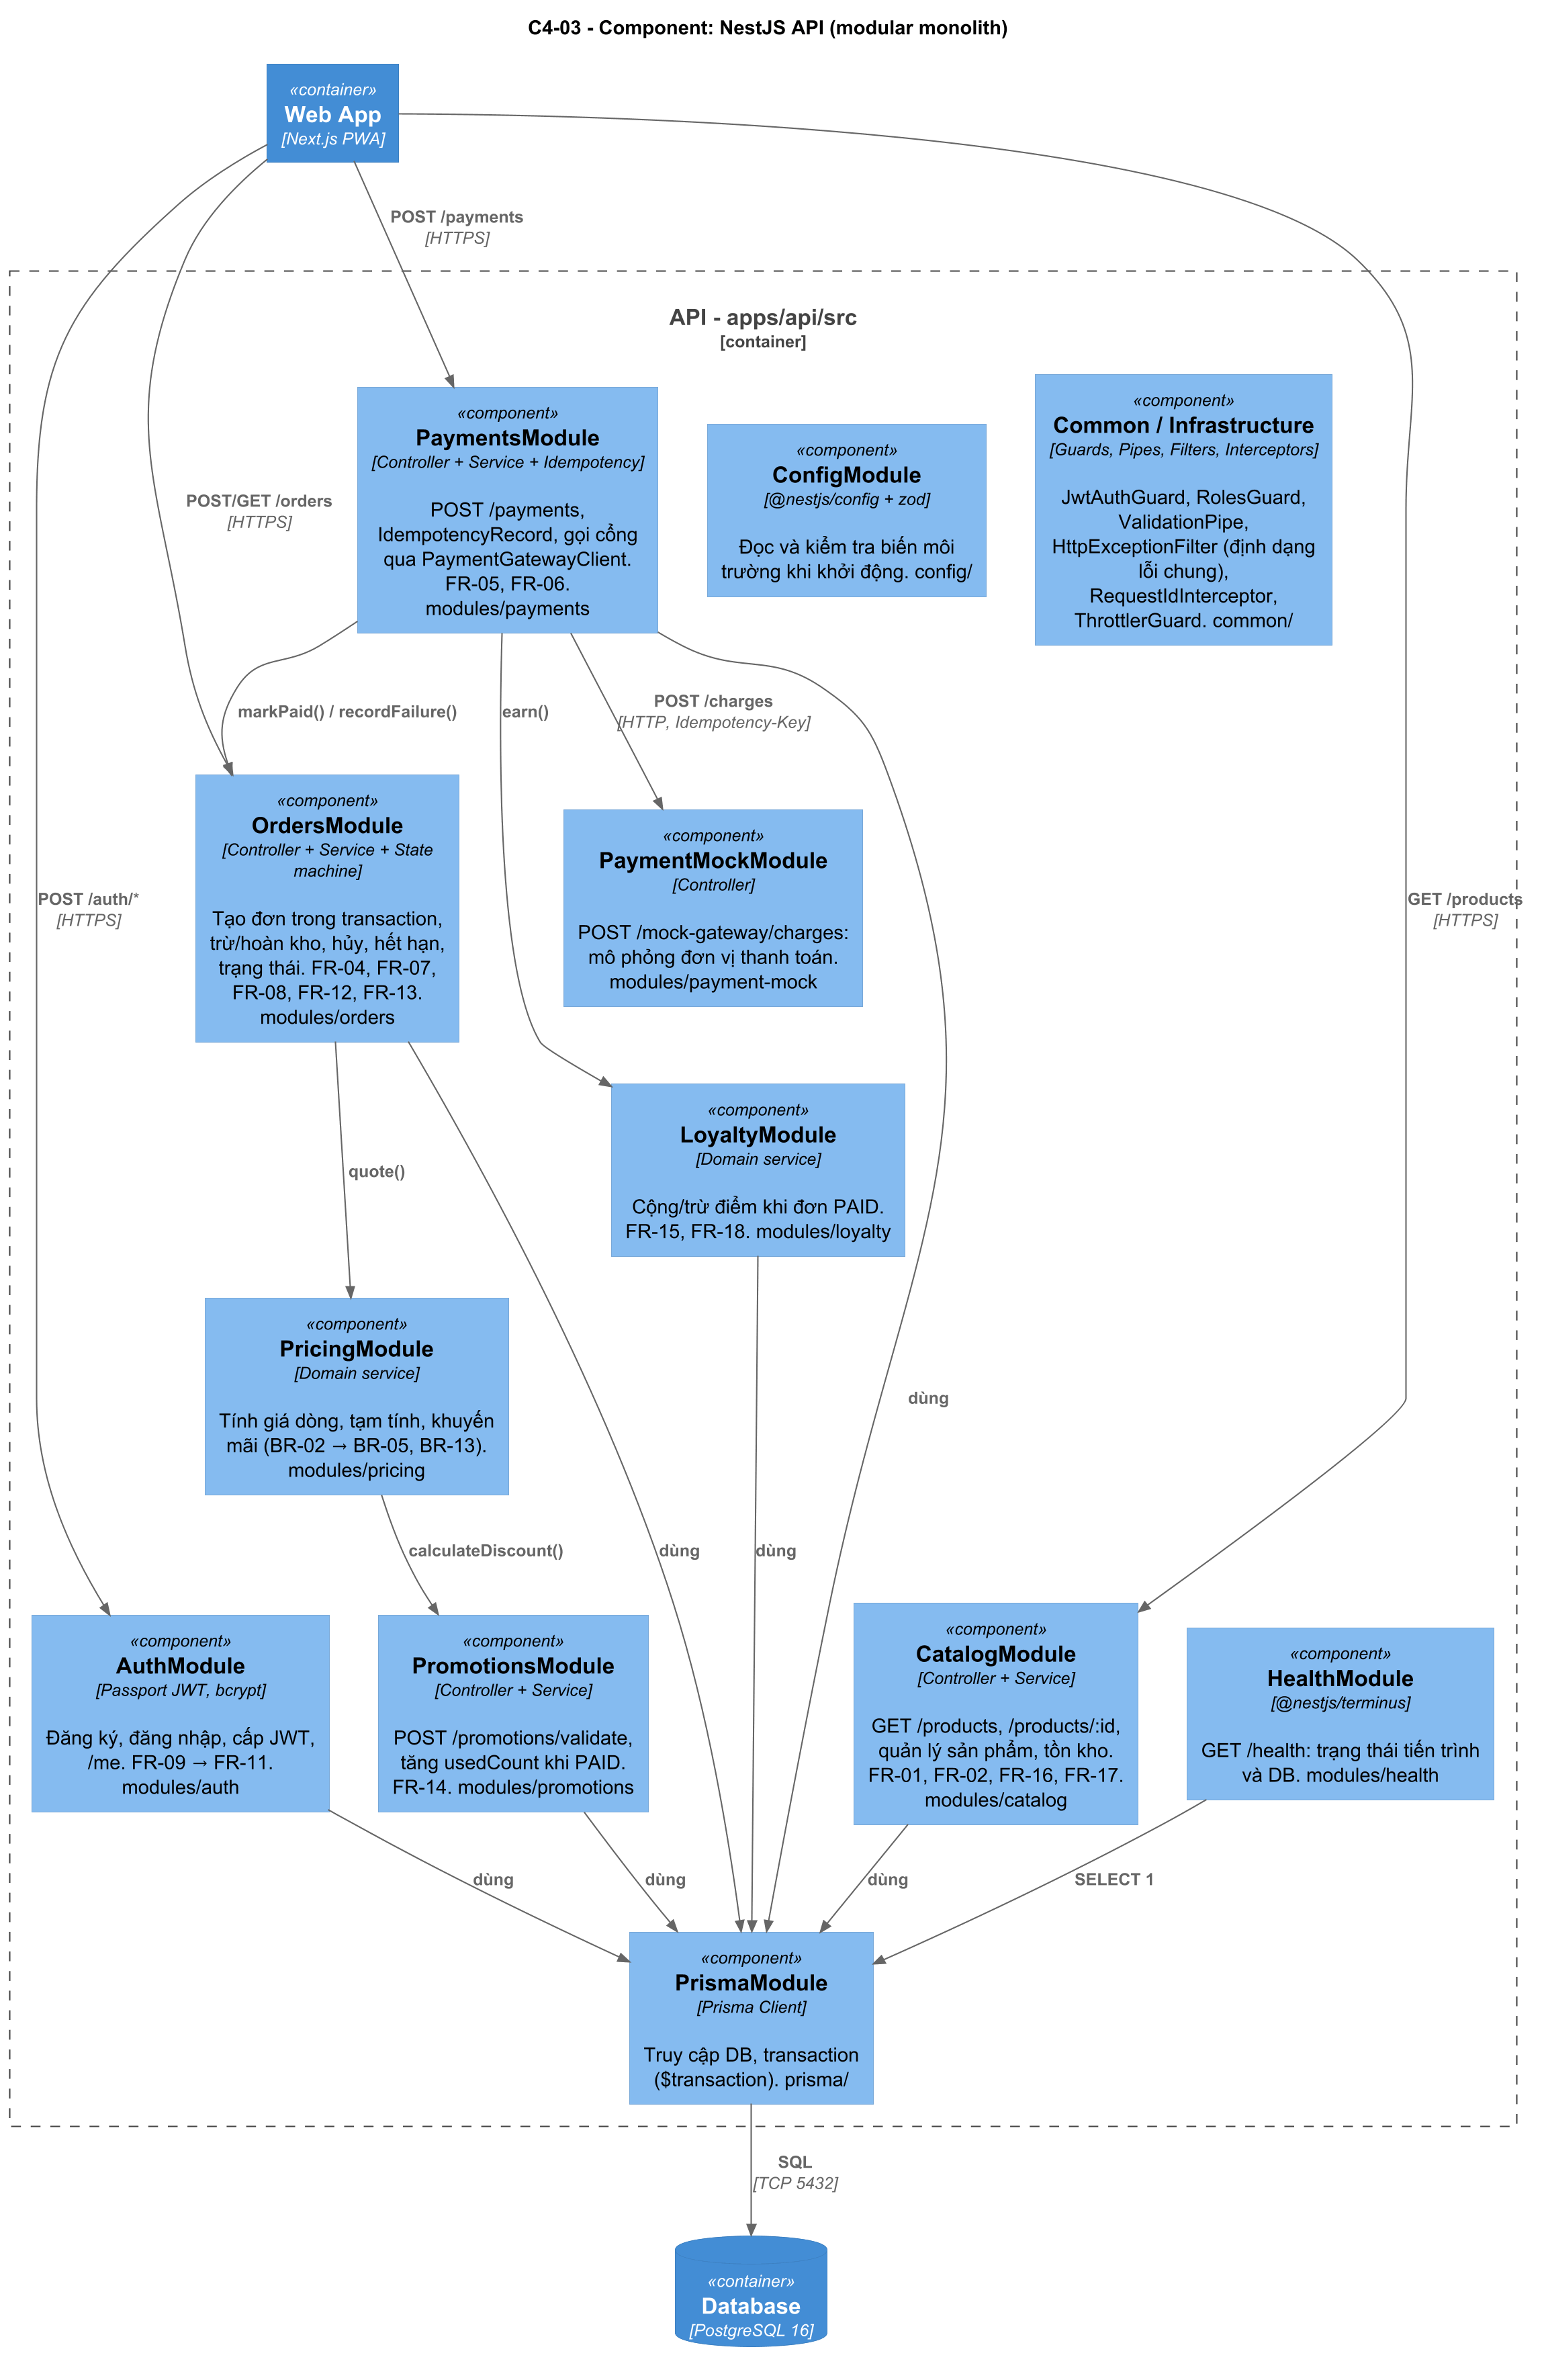
\includegraphics[width=\textwidth,height=0.82\textheight,keepaspectratio]{figures/c4-component-api.png}
\caption{C4-03 -- Component của NestJS API (modular monolith)}\label{fig:c4-component}
\end{figure}

\newpage
\subsubsection{Động lực kiến trúc}

\begin{longtable}{|p{2.4cm}|p{4.6cm}|p{7.8cm}|}
\caption{Động lực kiến trúc}\label{tab:drivers}\\
\hline
\thead \textbf{Mã} & \textbf{Động lực} & \textbf{Ảnh hưởng tới kiến trúc} \\ \hline
\endfirsthead
\hline
\thead \textbf{Mã} & \textbf{Động lực} & \textbf{Ảnh hưởng tới kiến trúc} \\ \hline
\endhead
C1 & Bắt buộc Next.js, NestJS, PostgreSQL & Ba container chính cố định \\ \hline
C9, C11 & 0 đồng, một người làm & Modular monolith thay vì microservices; dùng nền tảng có gói miễn phí \\ \hline
NFR-13, BR-07 & Không bán vượt kho & Trừ kho bằng \code{UPDATE ... WHERE stock >= qty} trong transaction \\ \hline
FR-06, BR-10, BR-11 & Không trừ tiền hai lần & Bảng \code{idempotency\_records} + unique index; Payment Service mô phỏng cũng idempotent \\ \hline
NFR-04 $\rightarrow$ 08 & Bảo mật & JWT, bcrypt, validate whitelist, Helmet, rate limit, CORS, secret qua biến môi trường \\ \hline
NFR-09, NFR-11 & Mobile-first, PWA & Next.js App Router + service worker \\ \hline
NFR-14 $\rightarrow$ 17 & Health, Docker, CI/CD & \code{/health}, Dockerfile mỗi app, image lên GHCR, deploy tự động \\ \hline
NFR-19 & Logging & Log JSON có \code{requestId}, che dữ liệu nhạy cảm \\ \hline
\end{longtable}

\subsubsection{Các container và thành phần}

\begin{longtable}{|p{2.6cm}|p{4.6cm}|p{4.2cm}|p{3.0cm}|}
\caption{Container của BrewLite}\label{tab:containers}\\
\hline
\thead \textbf{Container} & \textbf{Công nghệ} & \textbf{Trách nhiệm} & \textbf{Mã nguồn} \\ \hline
\endfirsthead
\hline
\thead \textbf{Container} & \textbf{Công nghệ} & \textbf{Trách nhiệm} & \textbf{Mã nguồn} \\ \hline
\endhead
Web App & Next.js App Router, React, TypeScript, TanStack Query, Zustand, Serwist, Tailwind CSS & Giao diện khách, nhân viên, quản lý; PWA & \code{apps/web} \\ \hline
API & NestJS, Prisma, Passport JWT, nestjs-pino, terminus & REST \code{/api/v1}, nghiệp vụ, transaction & \code{apps/api} \\ \hline
Payment Service (mô phỏng) & Module NestJS, HTTP & \code{POST /mock-gateway/charges} & \code{apps/api/src/} \code{modules/} \code{payment-mock} \\ \hline
Database & PostgreSQL 16 & Lưu trữ bền vững & \code{apps/api/prisma} \\ \hline
Shared (thư viện) & TypeScript, zod & Schema validate dùng chung & \code{packages/shared} \\ \hline
\end{longtable}

\paragraph{Frontend Next.js/PWA.} App Router; trang menu là Server Component để tải nhanh, phần tương tác là Client
Component. TanStack Query quản lý dữ liệu từ API (loading/error, retry), Zustand + \code{localStorage} giữ giỏ hàng,
react-hook-form + schema zod dùng chung với backend. Serwist tạo service worker: precache tài nguyên tĩnh, cache menu
kiểu \textit{stale-while-revalidate}, \textbf{không cache} API đơn hàng, thanh toán, xác thực; có trang offline.
\code{Idempotency-Key} được sinh khi bấm thanh toán và giữ trong \code{sessionStorage} tới khi có kết quả cuối.

\paragraph{Backend NestJS theo module/domain.} Các module \code{auth}, \code{catalog}, \code{pricing}, \code{orders},
\code{payments}, \code{loyalty}, \code{promotions}, \code{payment-mock}, \code{health}, cùng \code{prisma}, \code{config},
\code{common}. Mỗi module phân lớp Controller $\rightarrow$ Service $\rightarrow$ Domain logic thuần $\rightarrow$ Prisma.
Module chỉ gọi nhau qua service đã export; transaction dùng \code{prisma.\$transaction} và truyền transaction client cho
các service tham gia (ví dụ trừ kho khi tạo đơn).

\paragraph{PostgreSQL và migration.} Prisma quản lý schema và migration (commit trong
\code{apps/api/prisma/migrations}). Production chạy \code{prisma migrate deploy} khi container khởi động vì DB không
public. Quy tắc \textit{expand $\rightarrow$ contract} giúp rollback image không làm vỡ schema. Ràng buộc toàn vẹn:
\code{CHECK (stock >= 0)}, partial unique \code{payments(order\_id) WHERE status = 'SUCCEEDED'}, unique
\code{idempotency\_records(user\_id, key)}, unique \code{loyalty\_transactions(order\_id, type)}.

\paragraph{Dịch vụ thanh toán mô phỏng.} \code{PaymentMockModule} chạy cùng tiến trình API nhưng chỉ được gọi qua HTTP
bằng \code{PaymentGatewayClient} (\code{PAYMENT\_GATEWAY\_URL}, timeout 10 giây, header \code{Idempotency-Key}); lưu
giao dịch vào bảng \code{mock\_charges} để idempotent cả khi khởi động lại.

\paragraph{Logging, health check và cấu hình.} \code{nestjs-pino} ghi log JSON có \code{requestId} và che
\code{authorization}, \code{password}, số thẻ; \code{GET /health} ping DB, trả 200 hoặc 503; \code{ConfigModule}
kiểm tra biến môi trường bằng zod khi khởi động (fail fast); \code{.env.example} liệt kê đủ biến.

\subsubsection{Quyết định kiến trúc (ADR)}
Mỗi quyết định được ghi thành ADR ngắn trong \code{docs/architecture/adr/} theo mẫu Bối cảnh -- Quyết định --
Phương án đã cân nhắc -- Hệ quả.

\begin{longtable}{|c|p{4.4cm}|p{4.6cm}|p{4.6cm}|}
\caption{Tóm tắt ADR: lựa chọn và trade-off}\label{tab:adr}\\
\hline
\thead \textbf{ADR} & \textbf{Quyết định} & \textbf{Được} & \textbf{Mất / hạn chế} \\ \hline
\endfirsthead
\hline
\thead \textbf{ADR} & \textbf{Quyết định} & \textbf{Được} & \textbf{Mất / hạn chế} \\ \hline
\endhead
001 & Monorepo pnpm (\code{apps/web}, \code{apps/api}, \code{packages/shared}) & Schema dùng chung, một PR cho thay đổi xuyên tầng & Dockerfile build từ root; CI cần cache \\ \hline
002 & NestJS modular monolith, phân lớp theo module & Transaction DB cục bộ đúng và đơn giản; dễ unit test & Scale cả khối; cần kỷ luật ranh giới module \\ \hline
003 & Next.js App Router + PWA (Serwist) & SSR nhanh, cài được, có trang offline & Service worker có thể giữ bản cũ; không được cache API đơn hàng \\ \hline
004 & PostgreSQL + Prisma, migrate khi container khởi động & Migration có version; không cần mở DB ra ngoài & Phải tuân thủ expand/contract \\ \hline
005 & Payment mock cùng tiến trình, ranh giới HTTP & 0 chi phí, không cold start riêng, giữ hợp đồng HTTP + idempotency & Không độc lập về lỗi với API \\ \hline
006 & JWT Bearer HS256, 60 phút, bcrypt & Đơn giản, hợp CORS khác domain & Rủi ro XSS nếu lộ token; không thu hồi sớm \\ \hline
007 & Polling 3 giây cho trạng thái đơn & Chạy ổn mọi nền tảng, dễ test, đạt $\le$ 5 giây & Nhiều request hơn SSE \\ \hline
008 & pino JSON, \code{/health}, config zod & Truy vết theo \code{requestId}; fail fast & Log chỉ giữ theo gói miễn phí \\ \hline
009 & Vercel + Render + GHCR & HTTPS, CDN sẵn; DB nội bộ; rollback theo SHA & Cold start; Postgres free hết hạn 30 ngày \\ \hline
\end{longtable}

\subsubsection{Lý do chọn, ưu điểm và hạn chế}

\begin{table}[H]
\centering
\caption{Modular monolith so với microservices}\label{tab:monolith}
\begin{tabularx}{\textwidth}{|l|X|X|}
\hline
\thead \textbf{Tiêu chí} & \textbf{Modular monolith (chọn)} & \textbf{Microservices} \\ \hline
Công sức (1 người, 2 Sprint) & Thấp: một repo, một API, một DB & Cao: nhiều service, nhiều pipeline \\ \hline
Transaction đơn + kho + thanh toán & Transaction DB cục bộ, đúng (NFR-13) & Cần saga/outbox, khó đúng \\ \hline
Chi phí hạ tầng & 1 web service + 1 DB & Vượt gói miễn phí \\ \hline
Mở rộng độc lập & Hạn chế & Tốt \\ \hline
Khả năng tách sau này & Có: module ranh giới rõ, Payment qua HTTP & -- \\ \hline
\end{tabularx}
\end{table}

\textbf{Ưu điểm:} đơn giản, hợp quy mô; luồng chính dựa trên transaction DB nên dễ đảm bảo không bán vượt kho và
không trừ tiền hai lần; module ánh xạ 1--1 với nhóm FR; chạy local bằng một lệnh \code{docker compose up}.

\textbf{Hạn chế:} API và Payment Service mô phỏng chung tiến trình; Render free cho ngủ dịch vụ sau 15 phút (cold
start 30--60 giây); polling tốn request hơn SSE; frontend và API khác domain nên cần CORS và JWT lưu phía client.

%%%%%%%%%%%%%%%%%%%%%%%%%%%%%%%%%%%%%%%%%%%%%%%%%%%%%%%%%%%%%%%%%%%%%%
\newpage
\subsection{Task 3.2 -- Deployment diagram}

Production dùng nền tảng thực tế: \textbf{Vercel} cho Next.js, \textbf{Render} cho NestJS API (Docker image từ GHCR)
và PostgreSQL, \textbf{GitHub} cho mã nguồn, CI/CD và container registry. Sơ đồ thể hiện cả ba ranh giới Local, CI
và Production. Bản vector đầy đủ: \code{docs/architecture/diagrams/deployment.svg}.

\begin{figure}[p]
\centering
\begin{adjustbox}{angle=90,max width=\textwidth,max totalheight=0.9\textheight}
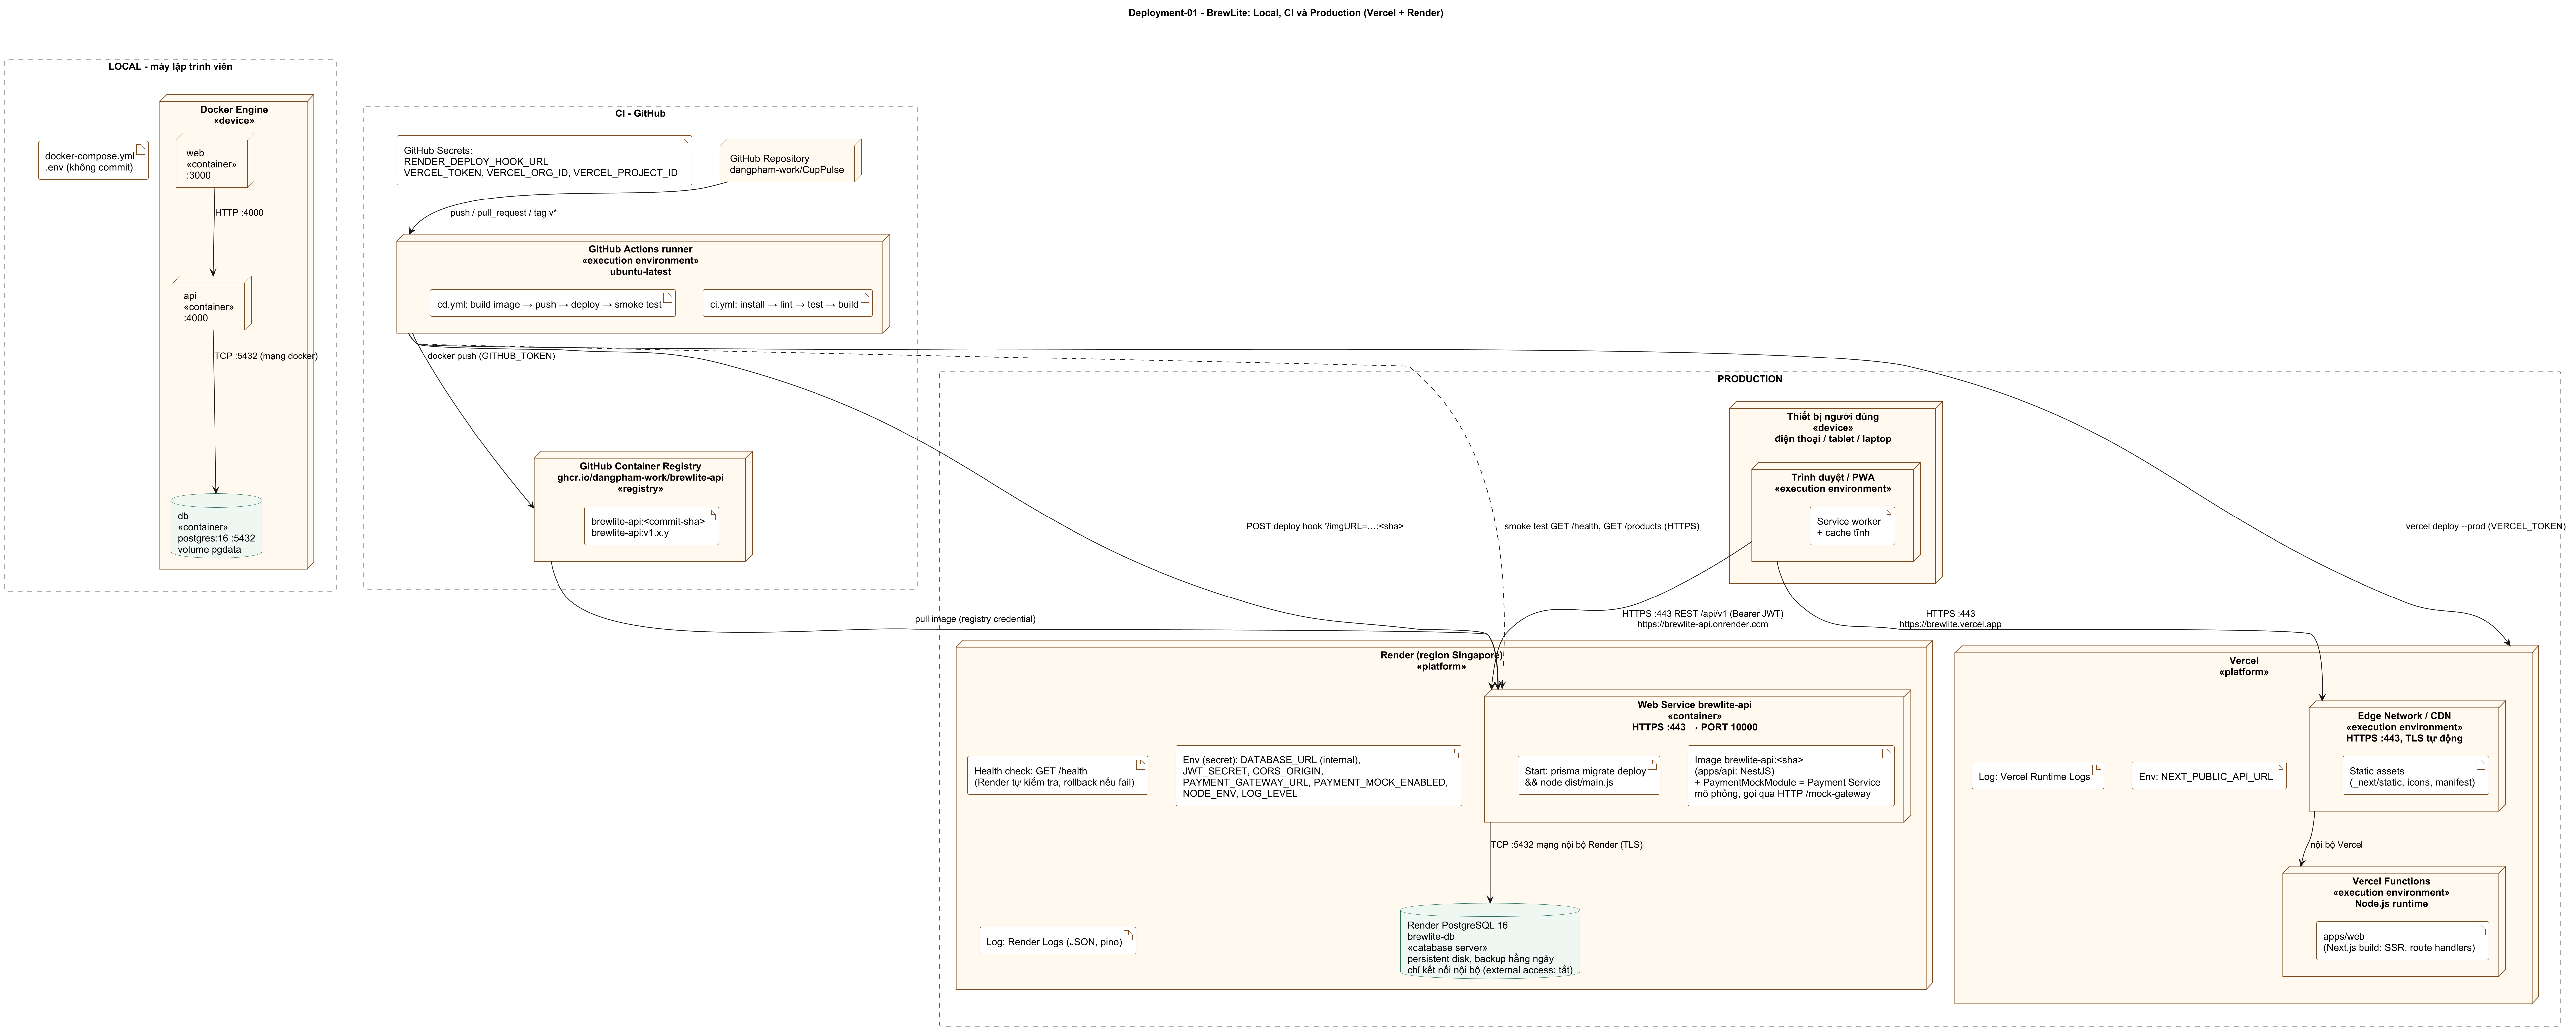
\includegraphics{figures/deployment.png}
\end{adjustbox}
\caption{Deployment-01 -- Local, CI và Production (Vercel + Render)}\label{fig:deployment}
\end{figure}

\begin{longtable}{|p{4.2cm}|p{4.4cm}|p{6.2cm}|}
\caption{Truy vết node triển khai $\rightarrow$ kiến trúc $\rightarrow$ mã nguồn}\label{tab:deploy-trace}\\
\hline
\thead \textbf{Node / artifact} & \textbf{Container C4 / thành phần} & \textbf{Mã nguồn / cấu hình} \\ \hline
\endfirsthead
\hline
\thead \textbf{Node / artifact} & \textbf{Container C4 / thành phần} & \textbf{Mã nguồn / cấu hình} \\ \hline
\endhead
Trình duyệt / PWA, service worker & Web App (client) & \code{apps/web/src/app/sw.ts}, \code{manifest.webmanifest} \\ \hline
Vercel Edge Network / CDN & Web App (tài nguyên tĩnh) & \code{apps/web/public/}, \code{.next/static} \\ \hline
Vercel Functions & Web App (SSR) & \code{apps/web/}, \code{vercel.json} \\ \hline
Render Web Service \code{brewlite-api} & API & \code{apps/api/}, \code{apps/api/Dockerfile} \\ \hline
Image \code{brewlite-api:<sha>} & API + PaymentMockModule & \code{.github/workflows/cd.yml} \\ \hline
Start \code{prisma migrate deploy} & PrismaModule, migration & \code{apps/api/prisma/migrations/}, \code{docker-entrypoint.sh} \\ \hline
Health check \code{GET /health} & HealthModule & \code{apps/api/src/modules/health/} \\ \hline
Render PostgreSQL \code{brewlite-db} & Database & \code{apps/api/prisma/schema.prisma} \\ \hline
GitHub Actions \code{ci.yml}, \code{cd.yml} & Quy trình CI/CD & \code{.github/workflows/} \\ \hline
GHCR \code{brewlite-api} & Registry của API & Tag do \code{cd.yml} gán \\ \hline
Docker Engine local (web, api, db) & Web App, API, Database & \code{docker-compose.yml}, \code{.env.example} \\ \hline
\end{longtable}

\begin{longtable}{|p{4.6cm}|p{4.0cm}|p{6.2cm}|}
\caption{Giao thức, cổng và kết nối}\label{tab:ports}\\
\hline
\thead \textbf{Từ $\rightarrow$ Tới} & \textbf{Giao thức / cổng} & \textbf{Ghi chú} \\ \hline
\endfirsthead
\hline
\thead \textbf{Từ $\rightarrow$ Tới} & \textbf{Giao thức / cổng} & \textbf{Ghi chú} \\ \hline
\endhead
Trình duyệt $\rightarrow$ Vercel & HTTPS 443 & TLS tự động; HTTP chuyển hướng HTTPS \\ \hline
Trình duyệt $\rightarrow$ Render API & HTTPS 443 & CORS chỉ cho domain Vercel \\ \hline
Render edge $\rightarrow$ container API & HTTP nội bộ, \code{PORT=10000} & TLS kết thúc tại Render \\ \hline
API $\rightarrow$ PostgreSQL & TCP 5432, mạng nội bộ, TLS & Internal Database URL; external access tắt \\ \hline
API $\rightarrow$ Payment Service mô phỏng & HTTP (\code{PAYMENT\_GATEWAY\_URL}) & Timeout 10 giây, \code{Idempotency-Key} \\ \hline
GitHub Actions $\rightarrow$ GHCR & HTTPS, \code{GITHUB\_TOKEN} & \code{docker push} \\ \hline
Render $\rightarrow$ GHCR & HTTPS, registry credential & Kéo image theo SHA \\ \hline
GitHub Actions $\rightarrow$ Render & HTTPS, deploy hook (secret) & \code{?imgURL=...:<sha>} \\ \hline
GitHub Actions $\rightarrow$ Vercel & HTTPS, \code{VERCEL\_TOKEN} & \code{vercel deploy --prod} \\ \hline
\end{longtable}

\begin{table}[H]
\centering
\caption{Secret và biến môi trường}\label{tab:secrets}
\begin{tabularx}{\textwidth}{|l|X|l|}
\hline
\thead \textbf{Nơi lưu} & \textbf{Biến} & \textbf{Ai đọc} \\ \hline
GitHub Secrets & \code{RENDER\_DEPLOY\_HOOK\_URL}, \code{VERCEL\_TOKEN}, \code{VERCEL\_ORG\_ID}, \code{VERCEL\_PROJECT\_ID} & \code{cd.yml} \\ \hline
Render Environment & \code{DATABASE\_URL} (internal), \code{JWT\_SECRET}, \code{CORS\_ORIGIN}, \code{PAYMENT\_GATEWAY\_URL}, \code{PAYMENT\_MOCK\_ENABLED}, \code{NODE\_ENV}, \code{LOG\_LEVEL} & Container API \\ \hline
Vercel Environment & \code{NEXT\_PUBLIC\_API\_URL} & Build Next.js \\ \hline
\code{.env} local (không commit) & Như \code{.env.example} & Docker Compose \\ \hline
\end{tabularx}
\end{table}

\textbf{Health check, log, rollback.} Render gọi \code{GET /health}; bản deploy mới không đạt thì bản cũ tiếp tục chạy.
Sau deploy, CI chạy smoke test \code{GET /health} và \code{GET /api/v1/products} có retry. Log API (pino JSON) xem ở
Render Logs, log web ở Vercel Runtime Logs. Rollback API bằng cách gọi lại deploy hook với image SHA trước đó; rollback
web bằng \code{vercel rollback}. Quy trình chi tiết sẽ nằm ở \code{docs/deployment.md} (Task 5).

\textbf{Giới hạn nền tảng.} Render free ngủ sau 15 phút (cold start, R8): smoke test có retry, ``đánh thức'' trước buổi
chấm. Render PostgreSQL free hết hạn sau 30 ngày (R1): nâng lên gói Basic (khoảng 6 USD/tháng) trước hạn hoặc tạo lại
DB rồi migrate + seed.
